\subsection{Benchmarking Rigs}
Two different systems were used:
\begin{compactitem}
\item a workstation A with an Intel Core Duo E8500 (\@ 3.16 GHz) CPU, 4 GB RAM, and a \cuda{} 2.1 capable NVIDIA GTX 560 Ti graphics card with 1 GB video memory
\item a workstation B with an Intel Xeon (\@ 2.53 GHz) CPU, 24 GB RAM, and an NVIDIA Tesla C2070 graphics card with 5 GB video memory
\end{compactitem}
All charts are marked accordingly.

\subsection{Using \lstinline!__restricted__! Pointers and References}
If all pointers and references in a function are marked as \lstinline!__restricted__!, the compiler assumes that there is no aliasing between them, that is that all pointers and references point to different memory locations.
Thus the compiler can better optimize the code and load more data directly into registers instead of having to use global memory accesses in sequence.

\subsection{Molecule Proxies}
The original code used a \lstinline!Molecule! structure to collection molecule data early on before calling the MoleculePairHandler. This was done to be independent of the actual molecule storage structures.
However, the \lstinline!Molecule! structure used a lot of memory and this resulted in big stack frames.
I rewrote it to use method accessor functions and act like a proxy to the molecule storage. It still wraps accesses and allows the molecule code to work without knowledge of the underlying storage but also uses less registers and local memory.

\subsection{Constant Memory}
Constant memory has its own 8 KB cache on each multiprocessor. Thus by moving constant data like the component descriptors, molecule interaction parameters and the storage buffer pointers into constant memory, global cache misses will be avoided and since this data is less than the size of the constant memory cache in total, it is likely that there will not be many constant memory cache misses.
Using constant memory results in a speed-up between 7 and 20 percent. See  \autoref{chart:no_constant_memory}.

\begin{chart}
\centering
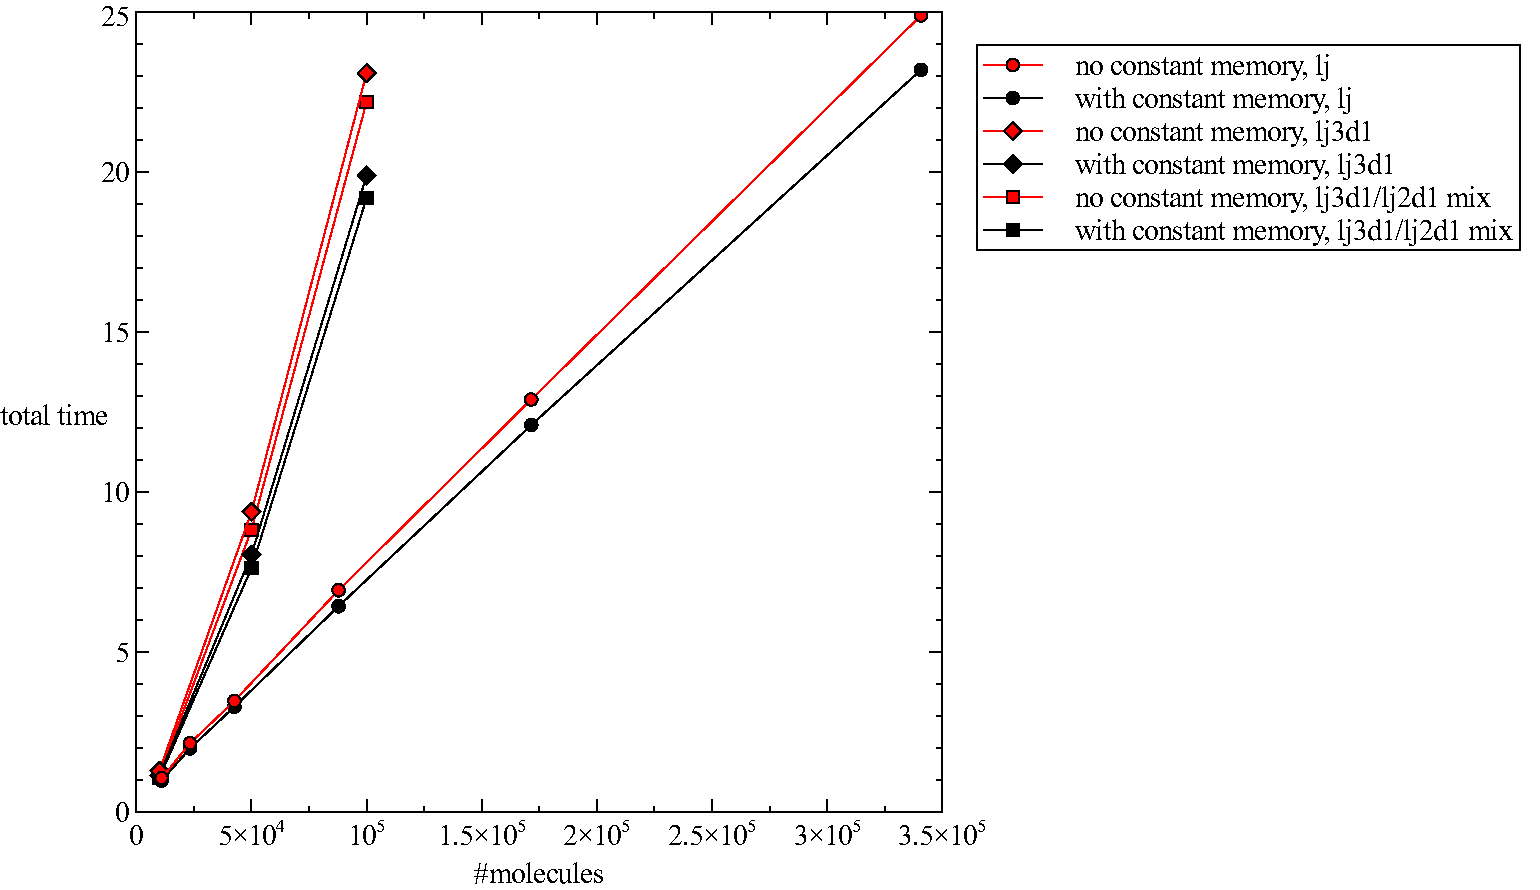
\includegraphics[width=0.75\textwidth]{plots/no_constant_memory.pdf}
\caption{constant memory speed-up (on workstation A)}
\label{chart:no_constant_memory}
\end{chart}

\subsection{Cells Sorted by Component Type}
\cuda{}'s performance decreases if threads inside the same warp take different branches because the SM has to serialize both code paths.
A simple but efficient optimization is to sort the molecules inside of each cell before calculating the interactions.
The current implementation simply loops over all molecules inside a cell once for each component type and writes them out in component type order.
This is inefficient but total execution time still improves visibly. See \autoref{chart:sorted_vs_unsorted}.

\begin{chart}
\centering
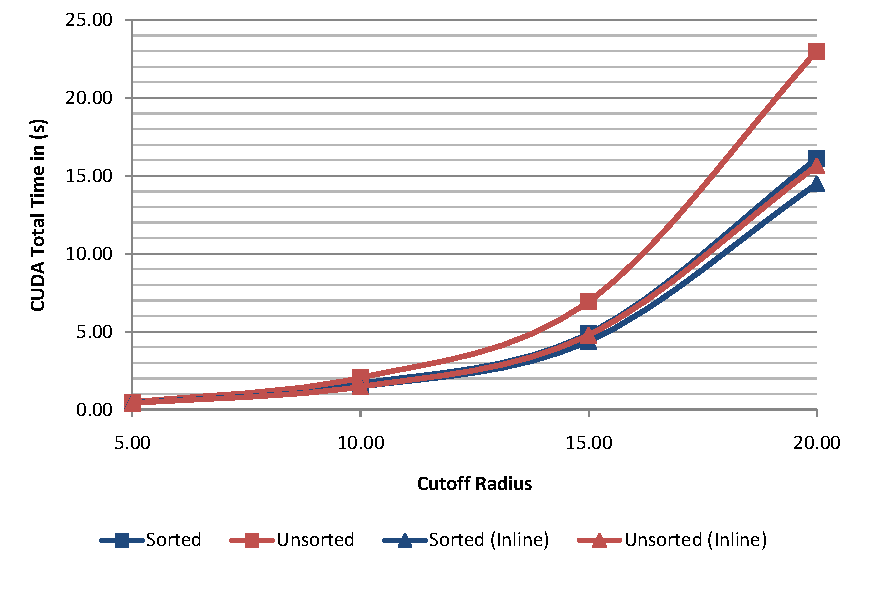
\includegraphics[width=0.75\textwidth]{plots/sorted_vs_unsorted.pdf}
\caption{cells sorted by component type speed-up (on workstation A). inline means that the pair handler function is being inlined (it usually is)}
\label{chart:sorted_vs_unsorted}
\end{chart}

\subsection{Without Effect: Non-Interleaved Molecule Data}
The \cite{cuda11bestpract} makes a strong point about the use of coalesced memory access. For additional insight on this, see \cite{volkov10}. The initial and currently used molecule storage code keeps the molecules stored in a semi-interleaved format:
\begin{lstlisting}[caption=Molecule Storage Declarations]
__constant__ __device__ floatType3 *moleculePositions;
__constant__ __device__ Quaternion *moleculeQuaternions;
__constant__ __device__ Matrix3x3 *moleculeRotations;

__constant__ __device__ floatType3 *moleculeForces;
__constant__ __device__ floatType3 *moleculeTorque;

__constant__ __device__ ComponentType *moleculeComponentTypes;

__constant__ __device__ uint *cellStartIndices;
\end{lstlisting}
The different fields (or streams) are stored non-interleaved but vector types are stored interleaved internally, that is the components are stored in sequence. I implemented fully non-interleaved version\footnote{every component of a vector, matrix or quaternion is stored in its own array} and tested it.

It actually runs slower. See \autoref{chart:packed_vs_unpacked}\footnote{\cudaConfigDouble{}}. My explanation for this is that the semi-interleaved version has better cache-locality. Even though each access on its own is not fully coalesced and has a stride, the next access can mostly use the same cache lines.
The non-interleaved version does not have this benefit.
\begin{chart}
\centering
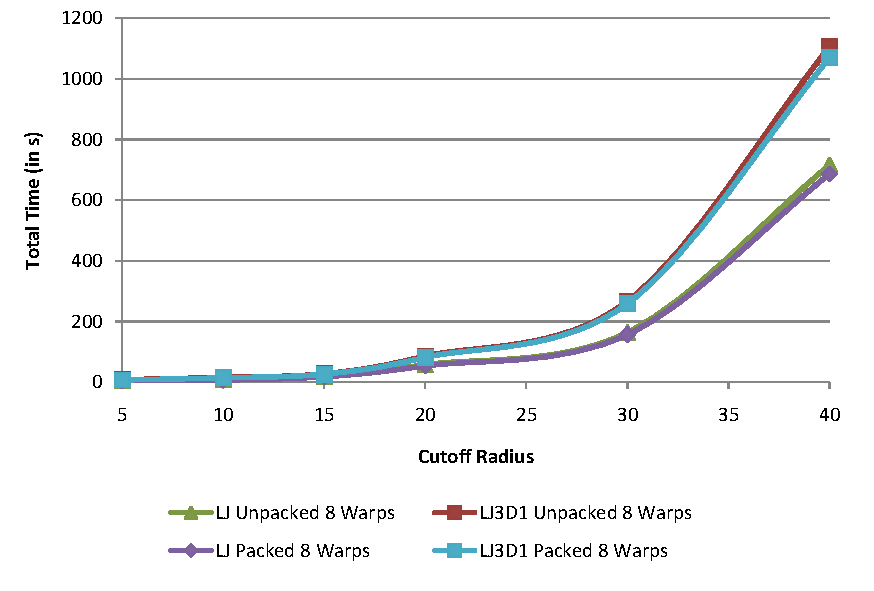
\includegraphics[width=0.75\textwidth]{plots/packed_vs_unpacked.pdf}
\caption{semi interleaved (packed) vs non-interleaved (unpacked) molecule storage (on workstation B)}
\label{chart:packed_vs_unpacked}
\end{chart}